\documentclass[11pt, headsepline]{article}

\usepackage[top=1in, bottom=1in, left=1in, right=1in]{geometry}
\usepackage{parskip}
\usepackage[colorlinks=true,linkcolor=blue,citecolor=blue,urlcolor=blue]{hyperref}
\usepackage{booktabs, cellspace, hhline, multirow, nicematrix}
\usepackage{float}
\usepackage{enumitem}
\usepackage{natbib}

\usepackage[usenames, dvipsnames]{xcolor}
\newcommand{\blue}[1]{\textcolor{blue}{#1}}
\newcommand{\red}[1]{\textcolor{red}{#1}}

\def\labelitemi{--}

\begin{document}

\section*{\centering \LARGE \normalfont Questionnaire}

\section*{Consent/screening}

\begin{enumerate}
    \item Thank you for your interest! We are a team of researchers from the University of Southern California conducting a study on economic preferences in the U.S. 
    The survey consists of multiple-choice and short-answer questions and will take approximately 15 minutes to complete.
    To participate, you must be a U.S. resident aged 18 or older. Do you confirm that you meet these criteria and would like to participate?

    Participation is voluntary, and you may exit the survey at any time. Your responses will be anonymous---no personally identifiable information will be retained, and you will not be personally identified in any findings. If you have any questions about the study, please contact us at nccarlso@usc.edu.

    \textit{Yes, I would like to participate and confirm that I am a U.S. resident aged 18 or older.; No, I do not wish to participate or do not meet the eligibility criteria.}
\end{enumerate}

\section*{Bot check}

\begin{enumerate}[resume]

    \item Please write the word “cactus” in the signature box below to confirm you are a human participant. This helps us ensure data quality. This is not a legal signature and will only be used for quality checks.

    [alternatively, ``banjo'']

    \textit{[signature box]}

\end{enumerate}

\section*{Age}

\begin{enumerate}[resume]

    \item What is your age?

    \textit{[text box]}

\end{enumerate}

\section*{Redistributive preferences}

\begin{enumerate}[resume]
    
    \item Should the government concern itself with reducing income differences between rich and poor people?

    \textit{The government should concern itself with this.; The government should not concern itself with this.}
    
    \item Should the federal income tax be more progressive than it is now (redistributing more income from the rich to the poor)?

    [Randomly shown to half of the participants at the end of the survey, before the Demographics section.]

    \textit{Much more progressive (lower earners should pay a lot less than they do now and higher earners should pay a lot much more than they do now); Somewhat more progressive; No change; Somewhat less progressive; Much less progressive (everyone should be taxed at about the same rate)}

    \item How have your views about redistribution of income (from the rich to the poor) changed over time? 

    \textit{I now support redistribution much more than in the past; I now support redistribution slightly more than in the past; No change; I now support redistribution slightly less than in the past; I now support redistribution much less than in the past; Other: [text box]}

    \item Why did your views on redistribution improve? 
    
    [Only displayed if the respondent answered that they now support redistribution ``slightly more'' or ``much more.'']

    \textit{Taxes affect me less now; I think the policy is better for the economy now; I think the policy is more fair now; Other: [text box]}

    \item Why did your views on redistribution worsen? 
    
    [Only displayed if the respondent answered that they now support redistribution ``slightly less'' or ``much less.'']

    \textit{Taxes affect me more now; I think the policy is worse for the economy now; I think the policy is less fair now; Other: [text box]}
    
\end{enumerate}


\section*{Tax proposal (randomized)}

\begin{enumerate}[resume]
    \item Imagine the government is considering reducing federal income taxes for lower earners and raising federal income taxes for higher earners. There will be no change in total government spending, because the increased tax payments by the higher earners offset the reduced tax payments by the lower earners. 
    
    The proposed policy is pictured in gray in the figure below. The percentages shown are effective personal income tax rates, which represent what the average person pays after deductions, exemptions and credits. The policy only involves federal income taxes, so the percentages shown in the figure do not include taxes for medicare and social security, or state/local taxes.

    [Participants will be randomly shown one of the following proposals.]

    \underline{Poor benefit}
    \begin{figure}[H]
        \centering
        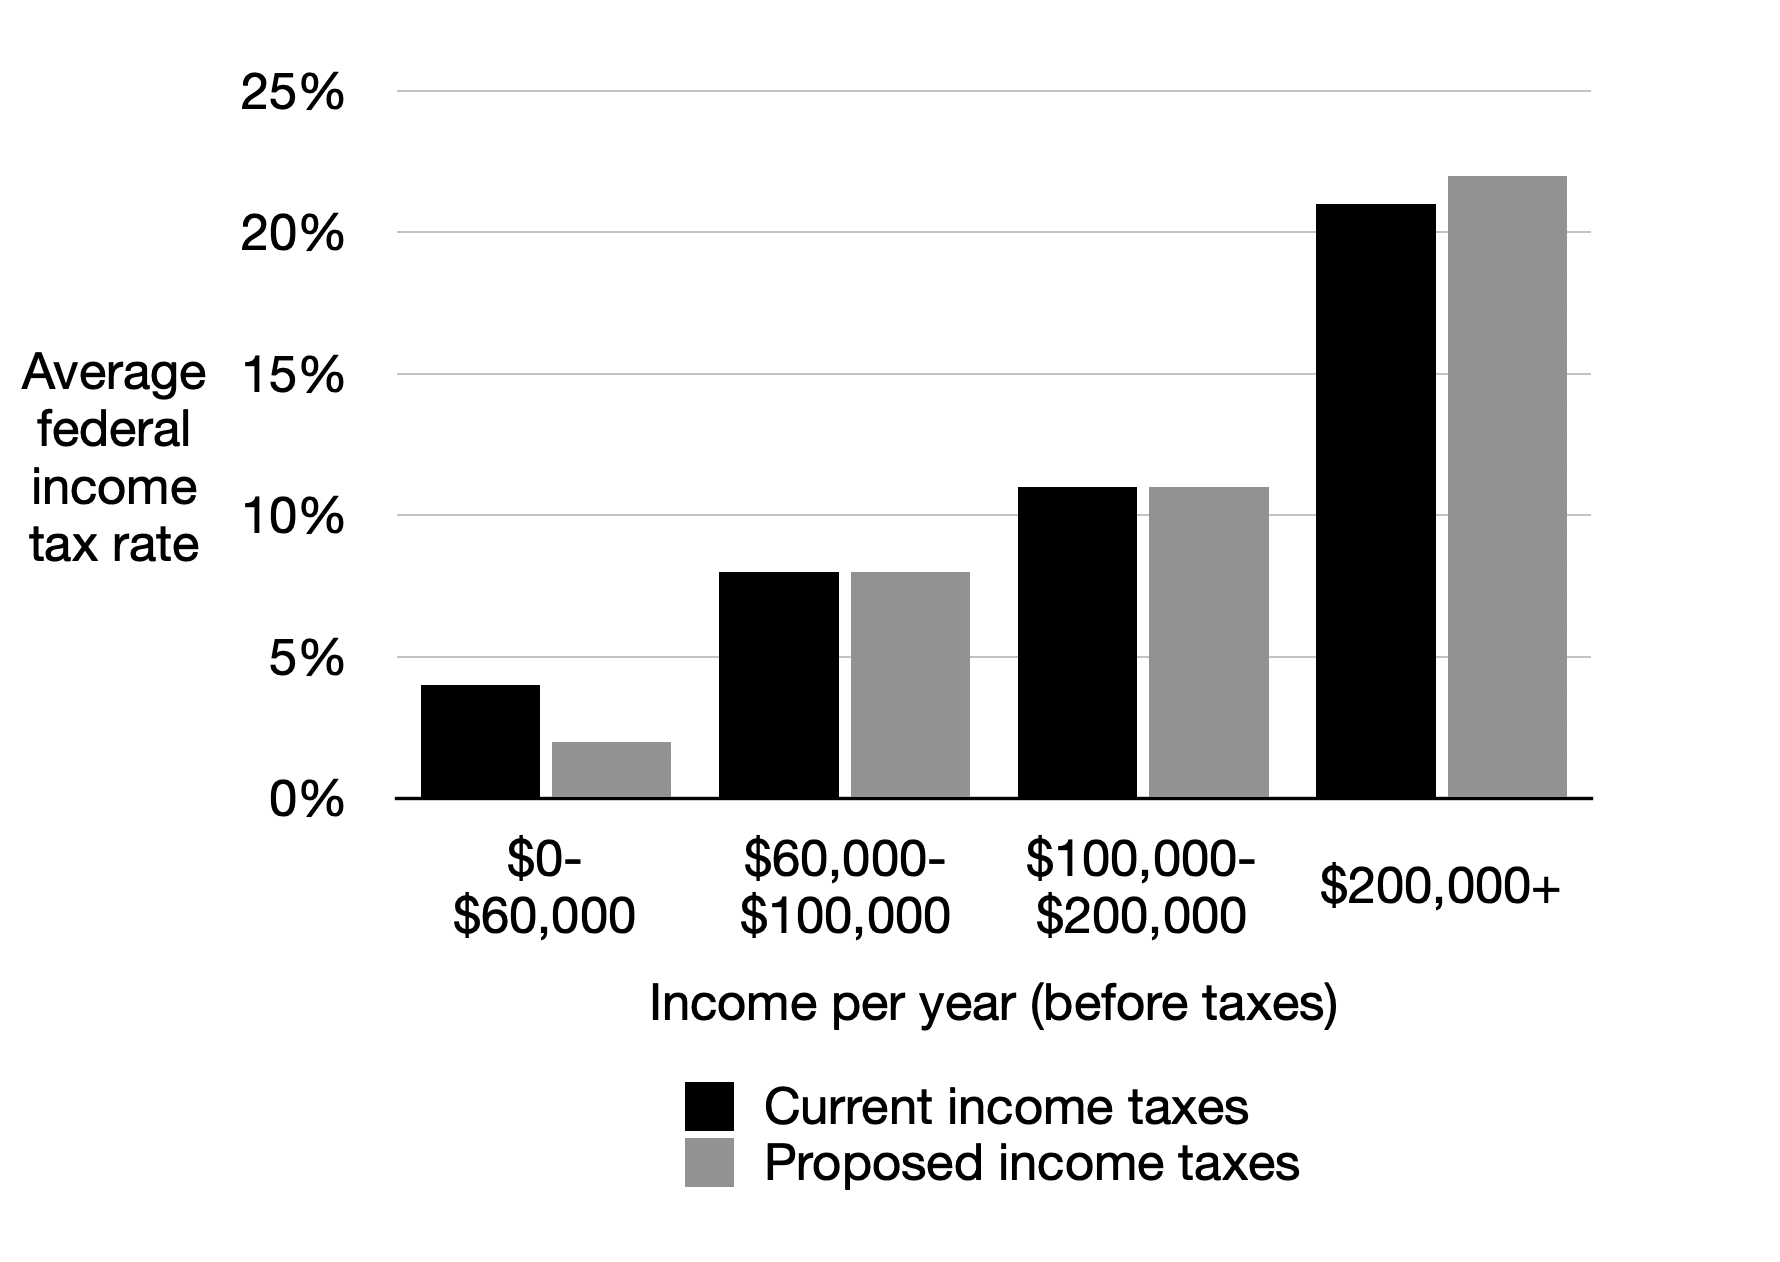
\includegraphics[width=0.7\linewidth]{images/poor.png}
        \label{fig:poor-benefit}
    \end{figure}
    \underline{Middle benefits}
    \begin{figure}[H]
        \centering
        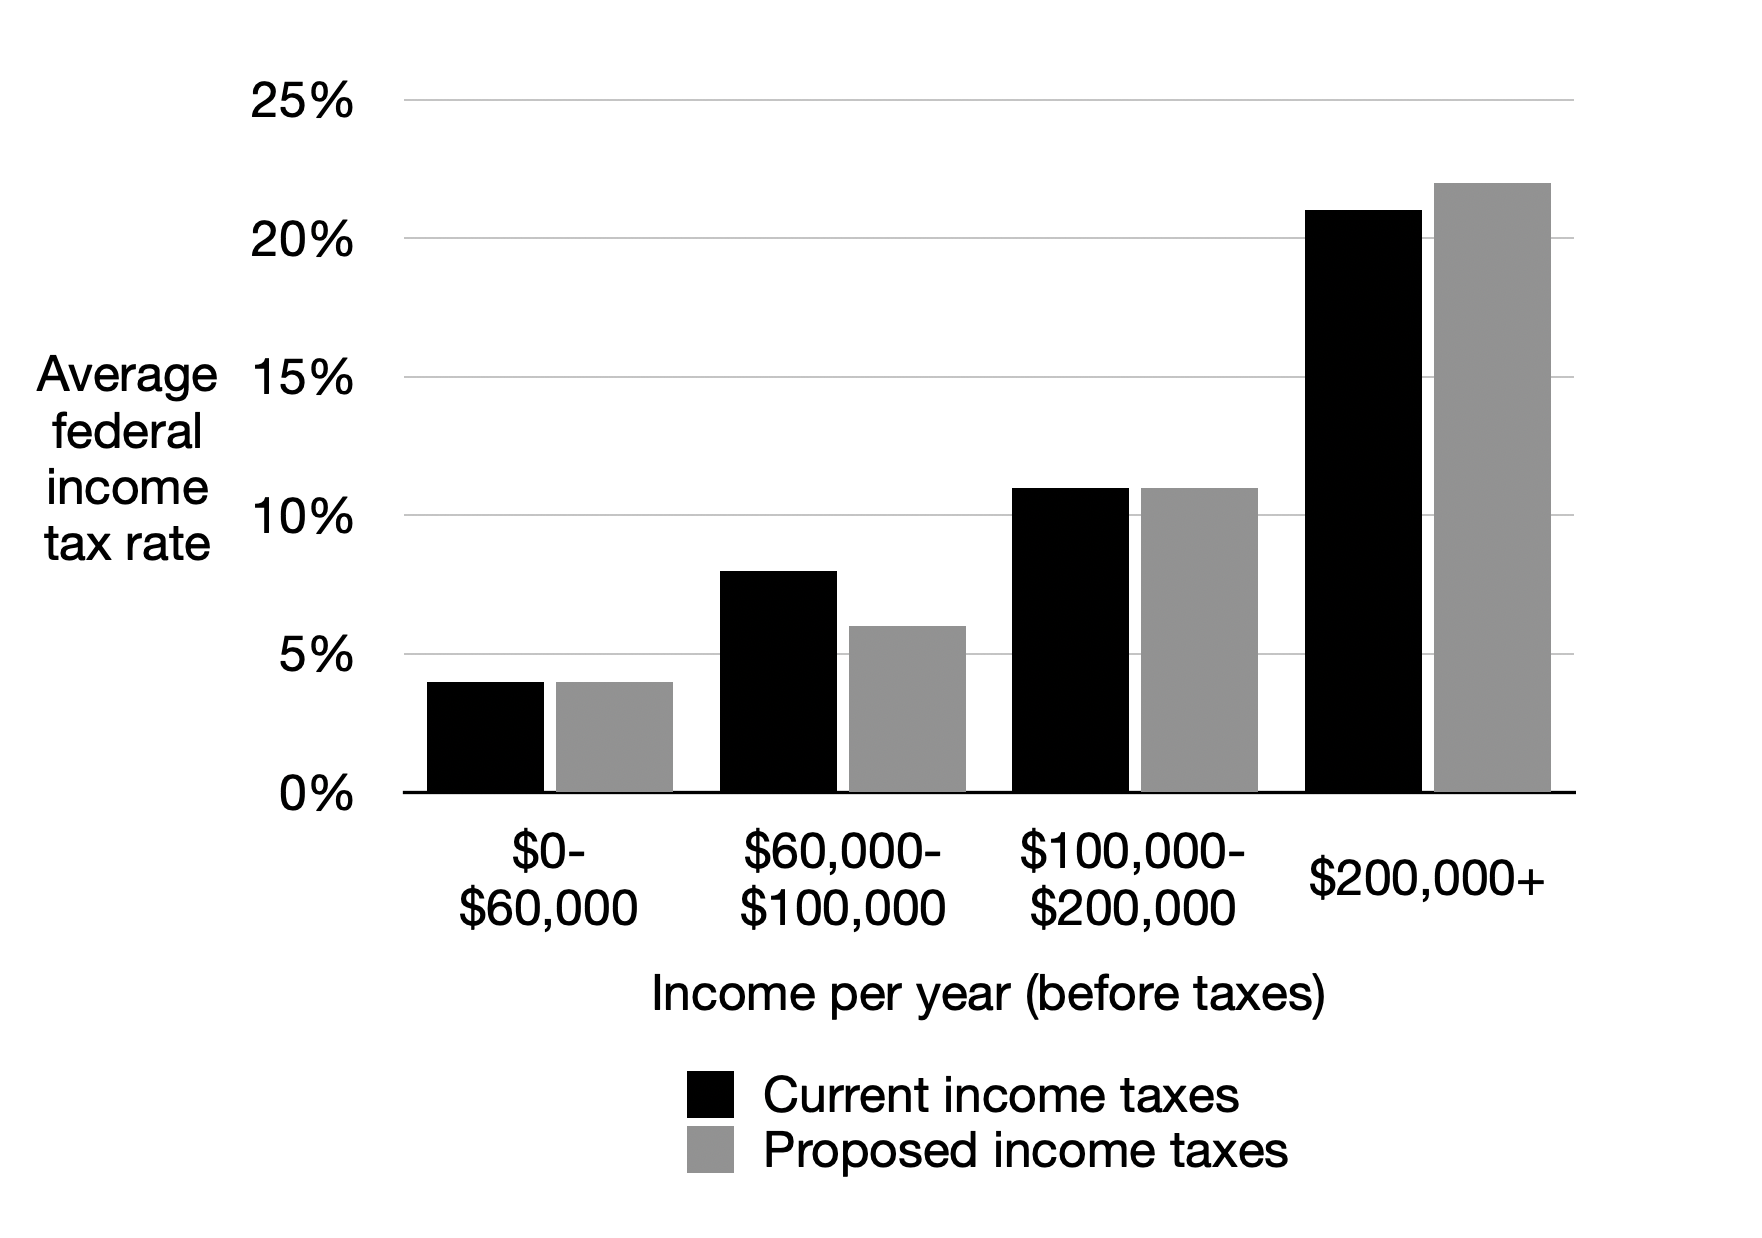
\includegraphics[width=0.7\linewidth]{images/middle.png}
        \label{fig:middle-benefit}
    \end{figure}
    \underline{Poor and middle both benefit}
    \begin{figure}[H]
        \centering
        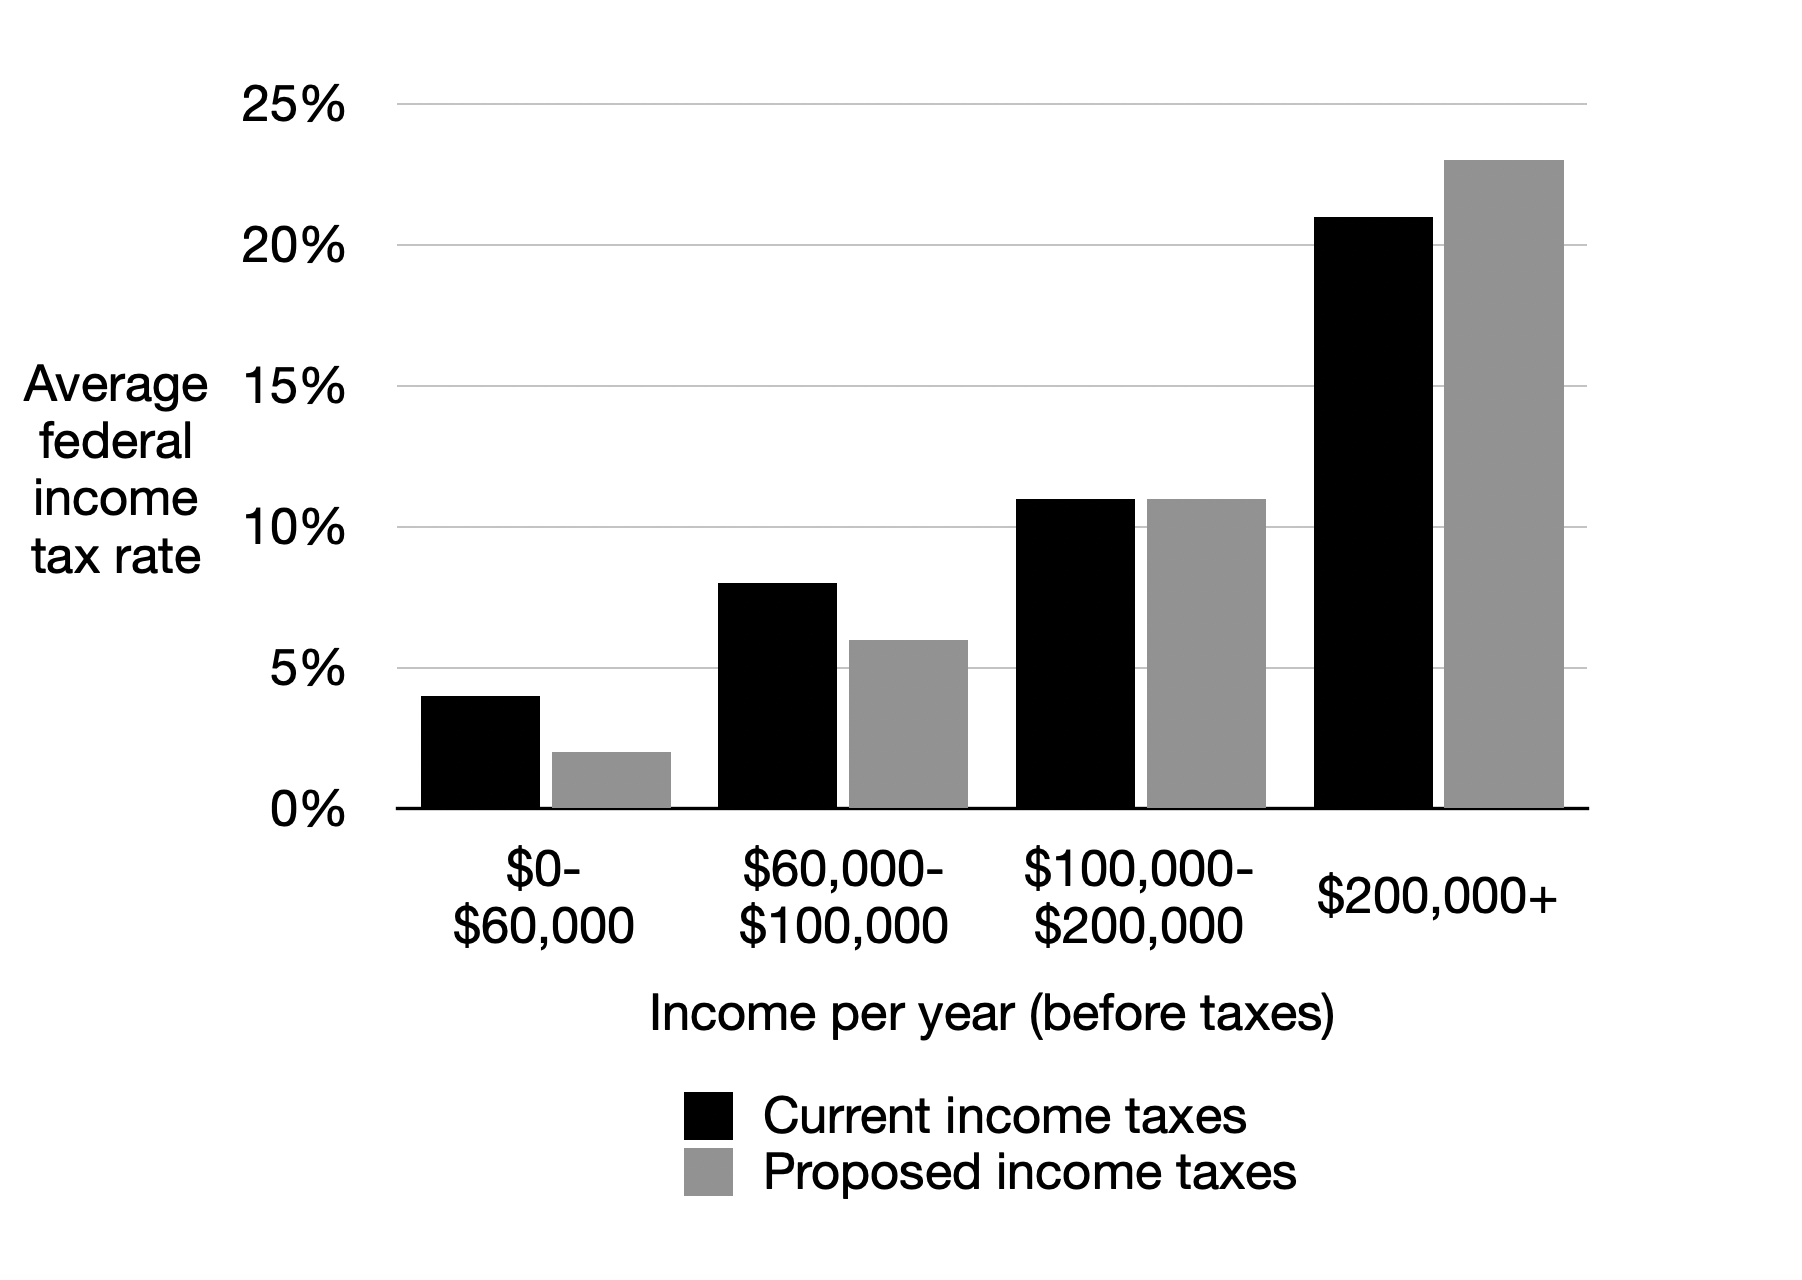
\includegraphics[width=0.7\linewidth]{images/both.png}
        \label{fig:both-benefit}
    \end{figure}

    Would you support or reject the proposed change?

    \textit{Support strongly; Support moderately; Support slightly; Indifferent; Reject slightly; Reject moderately; Reject strongly}
    
\end{enumerate}

\section*{Beliefs about incentive effects}

\begin{enumerate}[resume]
    \item If taxes on high incomes are increased and taxes on low incomes are decreased, people will not work as hard in their jobs.

    \textit{Agree strongly; Agree somewhat; Neutral; Disagree somewhat; Disagree strongly; Unsure}

    \item A large income gap is needed to motivate entrepreneurs to start businesses and innovate.

    \textit{Agree strongly; Agree somewhat; Neutral; Disagree somewhat; Disagree strongly; Unsure}
    
\end{enumerate}

\section*{Alternative policies}

\begin{enumerate}[resume]
    \item To support lower-income and middle-income Americans, the government should focus on improving education quality and access.

    \textit{Agree strongly; Agree somewhat; Indifferent; Disagree somewhat; Disagree strongly; Unsure}

    \item To support lower-income and middle-income Americans, the government should focus on protecting domestic jobs from international competition, for example, through tariffs.

    \textit{Agree strongly; Agree somewhat; Indifferent; Disagree somewhat; Disagree strongly; Unsure}

    \item To support lower-income and middle-income Americans, the government should focus on cutting taxes by reducing government services.

    \textit{Agree strongly; Agree somewhat; Indifferent; Disagree somewhat; Disagree strongly; Unsure}

    \item To support lower-income and middle-income Americans, the government should introduce publicly funded universal health insurance for all Americans (with the possibility to still purchase extra private insurance).

    \textit{Agree strongly; Agree somewhat; Indifferent; Disagree somewhat; Disagree strongly; Unsure}

    \item To support lower-income and middle-income Americans, the government should introduce a federal wealth tax on high-wealth individuals.

    \textit{Agree strongly; Agree somewhat; Indifferent; Disagree somewhat; Disagree strongly; Unsure}
    
\end{enumerate}

\section*{Zero-sum beliefs}

\begin{enumerate}[resume]

    \item People usually get rich at the expense of others rather than by creating value for others.

    \textit{Agree strongly; Agree somewhat; Neither agree nor disagree; Disagree somewhat; Disagree strongly; Unsure}

    \item In recent decades, large gains in CEO and executive salaries have been at the expense of the salaries of average workers.

    \textit{Agree strongly; Agree somewhat; Neither agree nor disagree; Disagree somewhat; Disagree strongly; Unsure}

    \item In recent decades, women’s wage gains have been at the expense of men’s wages.

    \textit{Agree strongly; Agree somewhat; Neither agree nor disagree; Disagree somewhat; Disagree strongly; Unsure}

    \item Diversity, equity, and inclusion (DEI) initiatives create opportunities for some at the expense of others.

    \textit{Agree strongly; Agree somewhat; Neither agree nor disagree; Disagree somewhat; Disagree strongly; Unsure}
    
\end{enumerate}

\section*{Current state of mobility and personal mobility}

\begin{enumerate}[resume]

    \item Consider a child coming from the poorest 20\% of families in the U.S. today. They are very determined and work hard in school, and later in life, they will work hard at their career. What do you believe is the chance that they make it into the richest 20\% of families/individuals when they are older?

    \textit{Almost guaranteed (80-100\%); Likely (60-80\%); Even chance (40-60\%); Unlikely (20-40\%); Almost no chance (0-20\%); Unsure}

    \item What do you believe is the chance that they make it into the richest 50\% of families/individuals when they are older?

    \textit{Almost guaranteed (80-100\%); Likely (60-80\%); Even chance (40-60\%); Unlikely (20-40\%); Almost no chance (0-20\%); Unsure}

    \item Is it harder or easier to move up in the U.S. now than when your parents were growing up (in terms of income/wealth)?

    \textit{Much harder now; Somewhat harder now; No change; Somewhat easier now; Much easier now; Unsure}

    \item Thinking about your past achievements, do you believe that your hard work in life has paid off or not?

    \textit{It has paid off a lot; It has paid off somewhat; It has not paid off much; Unsure}

    \item Thinking about your future achievements, do you believe that your hard work in life will pay off or not?

    \textit{It will pay off a lot; It will pay off somewhat; It will not pay off much; Unsure}

    \item Do you believe your education will pay off in terms of economic opportunity?

    \textit{It will pay off a lot; It will pay off somewhat; It will not pay off much; Unsure}
    
\end{enumerate}

\section*{Family mobility and relative income}

\begin{enumerate}[resume]

    \item When your mother (or first caretaker) was growing up, how did her (or their) family income compare to other American families?

    \textit{Far below average; Below average; Average; Above average; Far above average; Unsure / Not applicable}

    \item When your father (or second caretaker) was growing up, how did his (or their) family income compare to other American families?

    \textit{Far below average; Below average; Average; Above average; Far above average}

    \item When you were growing up, how did your family income compare to other American families?

    \textit{Far below average; Below average; Average; Above average; Far above average}

    \item Right now, how does your personal income compare with other Americans your age?

    \textit{Far below average; Below average; Average; Above average; Far above average}
    
\end{enumerate}

\section*{Income uncertainty}

\begin{enumerate}[resume]

    \item In the following questions, we will define personal income as income you earned yourself in a given year, and household income as the total income earned by yourself and any spouse, partner, or children under your care old enough to work. Income includes earnings from wages, self-employment, investment returns, pensions and retirement withdrawals.
    
    Are you the only person in your household or the only person earning income in your household?

    \textit{Yes; No, someone else also earns income}

    \item In 10 years, do you expect that more than one person in your household will be earning income? 

    \textit{Yes, more than one person; No, just myself}

    \item What was your total personal income (before taxes) last year (2024)?

    It is fine to approximate. Please enter a number such as 50,000 or 50000, but not \$50,000.

    \textit{[text box]}

    \item What do you expect your annual personal income (before taxes) to be 10 years from now?

    Please ignore inflation and answer using the value of a dollar today.

    \textit{[text box]}

    \item How certain are you that your personal income will be close to this number?

    \textit{Very certain; Somewhat certain; Not very certain}

    \item Thinking ahead 10 years, what is the highest your annual personal income (before taxes) might be under good—but still realistic—circumstances?

    \textit{[text box]}

    \item Thinking ahead 10 years, what is the lowest your annual personal income (before taxes) might be under bad—but still realistic—circumstances?

    \textit{[text box]}

    [The following questions in this section appear according to the responses at the beginning.]

    \item What was your total household income (before taxes) last year (2024)?

    \textit{[text box]}

    \item What do you expect your annual household income (before taxes) to be 10 years from now? 

    \textit{[text box]}

    \item How certain are you that your household income will be close to this number?

    \textit{Very certain; Somewhat certain; Not very certain}

    \item Thinking ahead 10 years, what is the highest your annual household income (before taxes) might be under good—but still realistic—circumstances?

    \textit{[text box]}

    \item Thinking ahead 10 years, what is the lowest your annual household income (before taxes) might be under bad—but still realistic—circumstances?

    \textit{[text box]}
    
\end{enumerate}

\section*{Perceived future income needs}

\begin{enumerate}[resume]
    \item At least how much annual household income (before taxes) would you need to live comfortably now?

    \textit{[text box]}

    [The following questions in this section appear only if the respondent is under 30 years old.]
    
    \item Is it more likely that you will or  will not have children to support in your 30s?

    \textit{Will have children; Will not have children}

    \item Assuming your answer to the previous question becomes true, how much annual household income (before taxes) will you need to live comfortably in your 30s?

    \textit{[text box]}

    \item Is it more likely that you will or will not have children to support in your 40s?

    \textit{Will have children; Will not have children}

    \item Assuming your answer to the previous question becomes true, how much annual household income (before taxes) will you need to live comfortably in your 40s?

    \textit{[text box]}
    
\end{enumerate}

\section*{Generosity and universalism}

\begin{enumerate}[resume]

    \item Imagine you unexpectedly receive \$100 as a gift. You have the option to keep all of it for yourself or give some of it to a complete stranger who is struggling to afford basic necessities. The money cannot be given to anyone else or donated elsewhere.

    How much of the \$100 would you choose to give to the stranger?

    \textit{[text box]}

    \item Imagine again that you unexpectedly receive \$100 as a gift. You have the option to keep all of it for yourself or give some of it to a friend or family member. The money cannot be given to anyone else or donated elsewhere.

    How much of the \$100 would you choose to give to a friend or family member?

    \textit{[text box]}
    
\end{enumerate}

\section*{Time discounting}

\begin{enumerate}[resume]

    \item Would you prefer \$1,000 today or \$1,100 in 1 year?

    \textit{\$1,000 today; \$1,100 in 1 year; Indifferent}

    \item Would you prefer \$1,000 today or \$1,500 in 1 year?

    \textit{\$1,000 today; \$1,500 in 1 year; Indifferent}

    \item Would you prefer \$1,000 today or \$2,000 in 1 year?

    \textit{\$1,000 today; \$2,000 in 1 year; Indifferent}

    \item Would you prefer \$1,000 today or \$1,100 in 5 years?

    \textit{\$1,000 today; \$1,100 in 5 years; Indifferent}

    \item Would you prefer \$1,000 today or \$1,500 in 5 years?

    \textit{\$1,000 today; \$1,500 in 5 years; Indifferent}

    \item Would you prefer \$1,000 today or \$2,000 in 5 years?

    \textit{\$1,000 today; \$2,000 in 5 years; Indifferent}

    \item I often prioritize my current needs and desires, even if it means delaying my long-term goals.

    \textit{Agree strongly; Agree somewhat; Indifferent; Disagree somewhat; Disagree strongly}
    
\end{enumerate}


\section*{Career plans and materialism}

\begin{enumerate}[resume]

    \item What do you value most in a job? Please rank top to bottom from most to least important by clicking or tapping on the choice tabs and dragging them up or down.

    \textit{Salary and benefits; Reasonable workload and/or flexible hours; Career growth and development; Meaningful and/or challenging work; Positive work environment and relationships}

    \item I would be satisfied with a modest income that covers basic needs—food, housing, clothing, healthcare, transportation—with a small amount left over for occasional extras.

    \textit{Agree strongly; Agree somewhat; Neutral; Disagree somewhat; Disagree strongly}

    \item Do you plan on starting a business at some point?

    \textit{Definitely / I have already started a business; Probably; Maybe; Probably not; Definitely not}

\end{enumerate}

\section*{Financial (in)security}

\begin{enumerate}[resume]

    \item How stable is your current primary source of income?

    \textit{Very stable; Somewhat stable; Neutral; Somewhat unstable; Very unstable}

    \item To what degree are you worried about losing your job or not finding a job?

    \textit{Very worried; Somewhat worried; Not very worried; Not worried at all}

    \item If you were to lose your job in the next 12 months, how likely is it that you would find a job with similar or higher pay within 3 months?

    \textit{Almost certain (90-100\%); Likely (60-90\%); Even chance (40-60\%); Unlikely (10-40\%); Almost no chance (0-10\%)}

    \item If you lost your source of income, how long could you maintain your current lifestyle using your financial safety net (savings and assets)?

    \textit{Less than 1 month; 1-3 months; 3-6 months; More than 6 months}

\end{enumerate}

\section*{Existential uncertainty}

\begin{enumerate}[resume]

    \item What is the risk of losing your job to artificial intelligence (AI) in the next 10 years?

    \textit{I have already lost a job to AI; The risk is high; The risk is substantial; The risk is low; No risk}

    \item What is the risk that you have to relocate due to climate events in the next 10 years?

    \textit{I have already relocated due to climate events; The risk is high; The risk is substantial; The risk is low; No risk}

    \item What is the risk that you have to live without health insurance in the next 10 years?

    \textit{I already live without health insurance; The risk is high; The risk is substantial; The risk is low; No risk}

    \item What is the risk that you are unable to ever own a home?

    \textit{The risk is high; The risk is substantial; The risk is low; No risk; I have already owned or currently own a home}

\end{enumerate}

\section*{Demographics}

Thank you for making it this far! To conclude, we would like to ask you some demographic questions.

\begin{enumerate}[resume]

    \item What is your gender?

    \textit{Male; Female; Non-binary; Prefer not to say}

    \item Please indicate your marital status.

    \textit{Single; Married; Cohabitating; Other: [text box]}

    \item How many children have you had?

    \textit{I do not have children; 1; 2; 3; 4; 5 or more}

    \item How many children in total do you plan on having over your lifetime?

    \textit{0; 1; 2; 3; 4; 5 or more; Unsure}

    \item How would you describe your ethnicity and/or race?

    \textit{American Indian or Alaska Native; Asian or Asian American; Black or African American; Hispanic or Latino; Middle Eastern or North African; Native Hawaiian or Pacific Islander; 
    White or European American; Other: [text box]}

    \item Were you born in the United States?

    \textit{Yes; No}

    \item Were both of your parents born in the United States?

    \textit{Yes; No}

    \item In which state do you currently reside? (If you are in college or temporarily stationed with the military, please enter the location you spend the most time in.)

    \textit{[state dropdown]}

    \item What is your current 5-digit ZIP code? (If you are in college or temporarily stationed with the military, please enter the location you spend the most time in. You may skip if you are not sure.)

    \textit{[text box]}

    \item Would you consider your current location urban, suburban, or rural?

    \textit{Urban; Suburban; Rural}

    \item Which state do you consider your home state (birthplace or place you grew up)?

    \textit{[state dropdown]}

    \item What is the name of your home town or city (birthplace or place you grew up)?

    \textit{[text box]}

    \item Would you consider your home town or city urban, suburban, or rural?

    \textit{Urban; Suburban; Rural}

    \item Are you a student right now?

    \textit{Not a student; High school; 2-year college; 4-year college; Master’s degree (e.g., MA, MS, MBA); Research doctoral program (e.g., PhD, DSc); Professional doctoral program (e.g., JD, MD)}

    \item Which category best describes your highest level education?

    \textit{Eighth grade or less; Some high school; High school degree / GED; Some college; 2-year college degree; 4-year college degree; Master’s degree (e.g., MA, MS, MBA); Research doctorate (e.g., PhD, DSc); Professional doctorate (e.g., JD, MD)}

    \item What is the highest level of education you plan on obtaining?

    \textit{Eighth grade or less; Some high school; High school degree / GED; Some college; 2-year college degree; 4-year college degree; Master’s degree (e.g., MA, MS, MBA); Research doctorate (e.g., PhD, DSc); Professional doctorate (e.g., JD, MD)}

    \item Which category best describes your mother's (or first caregiver's) highest level of education?

    \textit{Eighth grade or less; Some high school; High school degree / GED; Some college; 2-year college degree; 4-year college degree; Master’s degree (e.g., MA, MS, MBA); Research doctorate (e.g., PhD, DSc); Professional doctorate (e.g., JD, MD)}

    \item Which category best describes your father's (or second caregiver's) highest level of education?

    \textit{Eighth grade or less; Some high school; High school degree / GED; Some college; 2-year college degree; 4-year college degree; Master’s degree (e.g., MA, MS, MBA); Research doctorate (e.g., PhD, DSc); Professional doctorate (e.g., JD, MD)}

    \item What is your current employment status?

    \textit{Full-time employee; Part-time employee; Self-employed or small business owner; Unemployed and looking for work; Student; Not in the labor force (for example: retired, or full-time parent)}

    \item On economic policy matters, where do you see yourself on the liberal/conservative spectrum?
    
    \textit{Liberal; Moderate; Conservative}

    \item On social policy matters, where do you see yourself on the liberal/conservative spectrum?
    
    \textit{Liberal; Moderate; Conservative}

    \item Who did you vote for in the 2024 U.S. presidential election?

    \textit{Kamala Harris; Donald Trump; Other; I did not vote}

    \item Who did you vote for in the 2020 U.S. presidential election?

    \textit{Joe Biden; Donald Trump; Other; I did not vote}

\end{enumerate}

\section*{Feedback}

\begin{enumerate}[resume]

    \item Do you feel that this survey was left- or right-wing biased or unbiased?

    \textit{Left-wing biased; Right-wing biased; Unbiased}

    \item Let us know if you have any feedback—we're especially interested in whether any questions were confusing or if the survey length felt appropriate. Otherwise, we thank you for participating in the project!

    \textit{[text box]}
    
\end{enumerate}

\end{document}